In this section, we describe the currently discussed provenance data model. We 
start with the UML diagram and then give in the following sections more details 
for each class and relation.

\subsection{UML class diagram}
Figure \ref{fig:classdiagram} shows the UML diagram for an IVOA provenance data
model. It's core elements, which can also be found in the W3C provenance data
model are colored in blue. This pattern is very general and can be reused everywhere 
where provenance is needed. 

\begin{figure}[h]
\centering
\includegraphics[width=1.0\textwidth]{2016-05-03_IVOA_ProvenanceDM.png}
\caption{Class diagram for the provenance data model. The blue classes are core 
elements. Their names match the corresponding counterparts in the W3C provenance 
data model.}
\label{fig:classdiagram}
\end{figure}

\TODO{Produce Modelio version of the data model, update!}


\subsection{Core elements}\label{sec:core}
% Some examples for different use cases are given in Section \ref{sec:usecases-implementations}.
% The elements of a provenance model can be expressed as a directed graph to capture the causal dependencies. 

\begin{figure}[h]
\centering
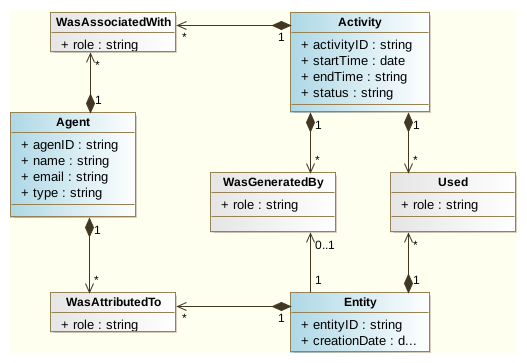
\includegraphics[width=0.8\textwidth]{../datamodel-diagrams/ProvDM-core-diagram.png}
\caption{The main core classes and relations of the Provenance Data Model, which also occur in the W3C model.}
\label{fig:coreclasses}
\end{figure}


The core elements of the provenance data model are Entity, Activity and Agent. 
We chose for these elements the same names as were used in the Provenance Data 
Model of the World Wide Web Consortium (W3C, \cite{std:W3CProvDM}), which defines 
a very abstract pattern that can be reused here. Here is a short description with 
some examples from the astronomy domain:

\begin{itemize}
\item \textbf{Entity:} a thing at a certain state\\
    examples: data products like images, catalogs, parameter files, calibration data, instrument characteristics

\item \textbf{Activity:} an action/process or a series of actions, occurs over a period of time, performed on or caused by entities, usually results in new entities\\
    examples: data acquisition like observation, simulation; regridding, fusion, calibration steps, reconstruction

\item \textbf{Agent:} executes/controls an activity, is responsible for an activity or an entity\\
    examples: telescope astronomer, pipeline operator, principal investigator, software engineer

\end{itemize}

\noindent

We use following relation classes to specify the mapping between the three core 
classes. The names were again chosen to match the W3C names:
\begin{itemize}
\item \textbf{WasGeneratedBy:} a new entitiy is generated by an activity\\
        (output\_data wasGeneratedFrom activity)
\item \textbf{Used:} an entity is used by an activity\\
        (activity used input\_data)
\item \textbf{WasAssociatedWith:} agents have responsibility for an activity\\
        (agent wasAssociatedWith activity)
\item \textbf{WasAttributedTo:} an entity can be attributed to an agent\\
		(entity wasAttributedTo agent)
\end{itemize}


\subsubsection{Entity}
Entities in astronomy are usually astronomical or astrophysical data sets in the form of images, tables, numbers, etc. But they can also be observation or simulation log files or, in a wider sense also observation proposals, scientific articles or manuals and other documents. An entity is not restricted to files. It can even be just a number in a table, depending on how fine-grained the provenance shall be described.

Entities in the VO are often called ``dataset'', which could mean a single 
table, an image or a collection of them. The Dataset Data Model 
\citep{std:DatasetDM} specifies an ``IVOA Dataset'' as ``a file or files which 
are considered to be a single deliverable''. We adopt this definition here and 
define ``Dataset'' as a subclass to Entity, as shown in Figure \ref{fig:entityclasses}.

\begin{figure}
\centering
\includegraphics[width=0.8\textwidth]{../datamodel-diagrams/ProvDM-entity-classes.png}
\caption{The Entity class and related subclasses}
\label{fig:entityclasses}
\end{figure}

For entities and datasets, we suggest the attributes given in Table \ref{tab:entity-attributes}. 
We use the namespace ``prov'', if the attribute also appears in ProvDM of W3C.

\begin{table}[h]

\small

\tymax	0.5\textwidth

\textbf{Entity}\vspace{0.25em}\\
\begin{tabulary}{1.0\textwidth}{@{}lp{3.5cm}lL@{}}
\toprule
\head{Attribute} & \head{Utype} & \head{Type} & \head{Description}\\
\midrule
\textbf{entityID} & DataID.observationID & string & a unique id for this entity (unique in its realm)\\
prov:label        & W3C model & string & a label (to be displayed by clients)\\
prov:type         & W3C model & string & a provenance type, i.e. one of: prov:collection, prov:bundle, prov:plan, not needed for a simple entity\\
\bottomrule
\end{tabulary}

\vspace{1cm}

\textbf{Dataset}\vspace{0.25em}\\
\begin{tabulary}{\textwidth}{@{}p{2.75cm}p{3cm}lL@{}}
\toprule
\head{Attribute} & \head{Utype} & \head{Type} & \head{Description}\\
\midrule
dataproduct\_type  & ObsDataset.data-ProductType & string       & from ObsCore data model \citep{std:ObsCore}, if applicable; describes, what kind of product it is (e.g. image, table)\\
calib\_level       & ObsDataset.calib-Level & enum integer & integer between 0 calibration level, if applicable, from ObsCore data model\\
%datatype           &                            & string       & type of the physical representation of the entity, e.g. binary file, fits file, database, database table, ASCII file, tar-file, directory, integer, float\\\hline
prov:description   & W3C model & string       & text describing the entity in more detail\\
prov:location or access\_url& W3C model & string & where the entity can be found/downloaded\\
access             & & string & values: public, restricted or internal\\
\bottomrule
\end{tabulary}

\caption{Attributes of entities and datasets. Mandatory attributes are marked as bold.}\label{tab:entity-attributes}
\end{table}

The difference between entities that are used as input data or output data 
becomes clear by specifying the relations between the data and activities producing/using these data.
More details on this will follow in Section \ref{sec:entity-activity-relations}.


\subsubsection{Collection}
Collections are datasets that are grouped together and can be treated as one single entity. 
In the provenance sense, they have some kind of common origin. The term ``Collection'' is 
also used in the Dataset Data Model for grouping datasets together, e.g. a collection 
with the name `RAVE survey' could consist of a number of database tables and spectra files.

The entity-collection relation can be modeled using the Composite design pattern: 
Collection is a subclass of Entity, but also an aggregation of 1 to many entities.

In order to be compliant to vodml, we model the membership-relation explicitely 
by including a `HadMember'' class in our model, which is connected to the
``Collection'' class via a composition. It may contain an additional role-attribute.

``Collection''s are also known in the W3C model, in the same sense as used here. 
The name for the mapping class, ``HadMember'' was adopted from the W3C model.

Advantages:
\begin{itemize}
\item use collections to provide overview, individual data for very detailed provenance; 
	  thus use collections for different levels of detail (granularity), hiding 
	  complexity where necessary
\item \TODO{Anything else?}
\end{itemize}

\TODO{Do we really gain that much?}
\TODO{Find a really strong use case for Collections to convince everyone that they are useful/needed.}


\subsubsection{Activity}
Activities in the VO include all steps in the reduction of images and production of new data sets, like image calibration, bias subtraction, image stacking; light curve generation from a number of observations, radial velocity determination from spectra, etc.

\begin{itemize}
\item For each data flow it should be possible to clearly identify entities and activities. If the activities shall not be recorded explicitely, one can also use the \emph{Derivation}-relation (see below) to link derived entities to their originals.

\item Data entities are results from activities (\emph{wasGeneratedBy}-relation), and can be used as input for other activities (\emph{used}-relation). 
%The difference between input data and output data becomes clear by specifying the relations. 

\end{itemize}

The W3C provenance model requires for activities an id, a startTime and endTime. 
Here's a list of useful further attributes for activities:

\begin{itemize}
\item id
\item prov:label
\item prov:type: one of the processes from a vocabulary or list, e.g. observation, reduction, calibration, publication
\item prov:description
\item prov:startTime
\item prov:endTime
\item docuLink: link to further documentation on this process, e.g. a paper, the source code in a version control system etc.
\end{itemize}

A ``version'' attribute could also be useful.

\subsection{Entity-Activity relations}\label{sec:entity-activity-relations}



\subsubsection{Agent}\label{sec:w3c-agent}
An agent can be an organization or a person, and can take different roles for an activity or an entity. The possible types of agents are:
\begin{itemize}
\item prov:person: a person, specified by first and last name, email address, possibly also by affiliation (though all these parts may change in time)
\item prov:organization: a publishing house, institute, scientific project
\item prov:SoftwareAgent: still needs to be discussed
\end{itemize}

A definition of organizations in the sense of the VO is given in the IVOA Recommendation on Resource Metadata \citep{std:ResourceMeta}, hereafter refered to as RM. This also specifies that scientific projects can be considered as organizations on a finer lever.

There can be more than one agent for each activity/entity (with different roles) and one agent can be responsible for more than one activity/entity. This many-to-many relationship could be made more explicite by adding role-maps for agents explicitely in the UML-class diagram, as ``qualifiers'' for the relations. The W3C PROV-DM document specifies two relations instead, which we can extend with a ``role'' attribute as well. These are:

\begin{itemize}
\item wasAssociatedWith: relates an \emph{activity} to an agent
\item wasAttributedTo: relates an \emph{entity} to an agent
\end{itemize}

Note that the attributed-to-agent for a dataset may be different from the agent that is associated with the activity that created an entity. Someone who is performing a task is not necessarily given full attribution, especially if he acts on behalf of someone else.

In order to make it clearer what an agent is useful for, we suggest here possible roles an agent can have (along with descriptions partially taken from RM)\\
\begin{center}
\begin{tabular}{l|l|p{0.5\textwidth}}
\multicolumn{3}{c}{\textbf{AgentRoles}}\\ \hline
\textbf{prov:role} & \textbf{prov:type} & \textbf{Comment} \\ \hline
author & prov:person & someone who wrote an article, software, proposal\\
contributor & prov:person & someone who contributed to something (but not enough to gain authorship)\\
curator & prov:person & someone who checked and corrected a dataset before publishing\\
editor & prov:person & editor of e.g. an article, before publishing\\
publisher & prov:organization & organization (publishing house, institute) that published something\\
observer & prov:person & observer at the telescope\\
operator & prov:person & performing a given task (executor?)\\
coordinator/PI & prov:person & someone coordinating/leading a proje'ct\\
provider & prov:organization & ``an organization that makes data and/or services available to users over the network'' (definition from RM)
%& prov:project & the project for which certain tasks are done, which published the data, etc.\\
\end{tabular}
\label{tab:agentroles}
\end{center}
This list is not complete. Such roles are domain-specific and thus not fixed in W3C's PROV-DM. However, since we are considering here the Astronomy-domain, we could 
consider fixing these roles, most likely by keeping them in a vocabulary list.

\TODO{Do we have a specific use case for fixing the agent-roles? Is anyone going to search for specific roles in the Provenance meta-data?
Or shall we leave it open, which roles can be defined and just give examples here?}

\TODO{Do we need to fix the prov:types to the given roles? Or leave it free?}

\TODO{We still need to clarify precisely, in which way a \emph{software agent} is distinct from an activity.}


\subsubsection{Roles of entities}
\TODO{Probably these roles are best stored with the used/wasGeneratedBy relation directly.}
The W3C PROV-DM specifies a \textbf{Derivation} relation, which directly links a derived entity to its predecessor. This was introduced to make the link between entities more explicite. If activity a1 used entities e1 and e2 as input and produced e3 as output, then it is not clear, if e3 is a derivative (or, in W3C terms, ``wasDerivedFrom'') of e1 or if it was derived from e2 or from both or neither. e1 and e2 could have been only parameter files for an observation.  

However, for the IVOA provenance model we currently favour adding a \emph{role} to each data item or entity, which can explain in more detail in which way the entity was used.

We will discuss later an approach using the additional Method-class as prototype or template for each activity.
The types of input/output data and their roles are described using additional classes for the method, so that any kind of relation between input/output data can be covered.

One of the important details here is that e.g. many data sets used by one activity may have different roles for that process (one file is a parameter file, another one is the raw image, and the third one is the dark field that should be subtracted). Since these roles are very important for an activity, they have to be included in the provenance model.

These roles don't have to be unique (see \cite{moreau2010}, after Definition 10), many data sets may have the same role for a process (e.g. raw image input).

Each activity requires specific roles for each entity (provided in the used- or wasGeneratedFrom-relation). 

\TODO{In order to facilitate interoperability, for each activity, the possible entity-roles could be defined and described by the IVOA community, in a vocabulary list or thesaurus.}



% The derivation relation together with entities is already enough to produce a data flow view, but in Astronomy we are probably even more interested in the Processes (as discussed in our first draft for requirements for provenance).



\subsubsection{Work flows: Plan and Bundle}
W3C suggests to use the term \emph{Plan} for entities that represent workflows and recipes. This could be interesting to include for workflow systems such as AstroTaverna. 

It could be used for grouping activities of a workflow together, e.g. when
the intermediate entities generated by the individual activities of the workflow shall not be described explicitely. The activities can be chained together in the correct order using W3C's ``wasInformedBy'' relation (also called ``Communication'' relation) in between.

Later on we will discuss that we could instead use a construct like an ``ActivityCollection'' for this.

``Bundles'' are used to name a set of provenance descriptions. It is a type for an entity, and allows to express provenance of provenance. This is probably also very interestíng for workflow systems.

\TODO{What about D-PROV for workflows?}

\subsubsection{Hierarchical descriptions}
OPM also suggests to allow hierarchical descriptions, i.e. allow to include different ways of getting from dataset A to dataset B, with different levels of detail. 
This needs to be discussed further. 
%(After talk at InterOp-Madrid, May 2014, some people said that this would be important for them!)


\subsection{A model using prototypes}
Inspired by \cite{std:SimDM}, a data model for simulation data published in May 2012, we also discuss an IVOA provenance data model with prototypes. 
%Currently, we are still debating about this, but favour to follow the example of the W3C-model and postpone a decision for or against prototypes to a later version of this model. 
The W3C-model has the advantage of being already an approved standard, and it contains all the necessary main features needed for a Provenance model for Astronomy. However, it is very general, and by adding reusable prototypes, templates or descriptions for activities and entities,  the model may fit better to the astronomy domain.

It still remains to be seen if this is necessary, useful or just nice to have. Currently, we consider having prototypes in the model, for normalization purposes, but when serialising the provenance we could integrate the description side into the other classes, thus producing W3C compliant provenance.



\subsubsection{New classes from SimDM's provenance pattern}
From SimDM we adopt the pattern of two central classes: \emph{protocol} and \emph{experiment}.  A protocol is the plan or method
which describes how to do something, whereas experiment is the actual execution of
this plan. Defining such protocols allows them to be reused, which is very useful when performing series of experiments of the same type, as is typically done in astronomy. Comparing with the W3C terms, the experiment corresponds to an activity. Instead of protocol, we use the term \emph{description} or \emph{method}, 
for not confusing it with e.g. IVOA protocols.

A class diagram including this description-side %generated with MagicDraw Community Edition 
is given in Figure~\ref{fig:classes-prototypes}; the details are described in the following sections.

\begin{figure}
\centering
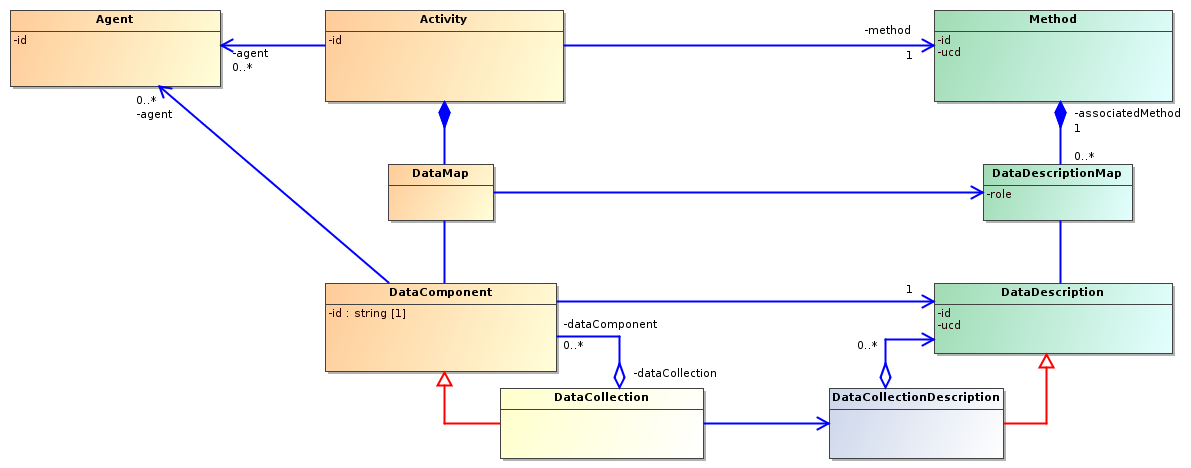
\includegraphics[width=0.8\textwidth]{ProvDM-classdiagram-prototypes.png}
\caption{The class diagram for a provenance data model including prototypes/descriptions for each activity and entity. It will certainly change again, so use it with care. In this version, we stripped it now from nearly all derived classes, so we can concentrate on the core elements. The green and blue boxes belong to ``prototype'' classes.}
\label{fig:classes-prototypes}
\end{figure}


\subsubsection{Activity and method}
As mentioned before, activity corresponds to experiment, and method to protocol from \cite{std:SimDM}.
Some examples for astronomical activities were already given at the beginning of this chapter. They are processes like observations, post-processing, flat-fielding, correcting bias, astrometric calibration, etc. The method underlying an activity is specified by the corresponding \emph{ActivityDescription} class (previously named \emph{Method}. This could be, for instance, the name of the code used to perform an activity or a more general description of the underlying algorithm. An activity is a concrete case (instance) of using such a method, with a startTime and endTime, and it has to refer to a corresponding method for further information. 

There MUST be exactly one ActivityDescription per Activity. If steps from a pipeline shall be 
grouped together, one needs to create a proper ActivityDescription for describing all 
the steps at once. This method can then be refered to by the pipeline-activity. For grouped activities, also see the next section.

\subsubsection{ActivityCollection}
For facilitating grouping of activities while still making it obvious that this group contains activities, we introduce an \emph{ActivityCollection}, and on its description side also an \emph{ActivityCollectionDescription}. This can be used for describing workflows, instead of using \emph{Plan} as suggested by the W3C model.

\TODO{More details here, why it is useful, what the description-side contains, what not ...}

\subsubsection{DataEntity and DataEntityDescription}
We define a general \emph{DataEntity} class, 
which can represent either an individual data item or a collection of data. The W3C equivalent to this class is called \emph{Entity} only, but we use here \emph{DataEntity} instead, since we do not aim to model cars and abstract ideas here, but more concretely astronomical data of any kind.

\TODO{Decide, if we want to stick to \emph{Entity} instead of \emph{DataEntity} for keeping 
compliance with W3C.}

Following the scheme that each \emph{activity} is described
by its more general \emph{method}, we associate each input or
output data set with a corresponding description of the dataproduct type. 
This just describes the data as it is, its format and content, and could be derived
from other IVOA data models like ObsCore for observations or SSA for spectra.
The DataEntityDescription does NOT contain any information about the usage of the data, 
it tells nothing about them being used as input or output.

\subsubsection{Input/output data, roles for data}
The information on whether data is used as input or was produced as output of 
some activity is given by the \emph{relation-types} between activities and entities.

Each method usually makes assumptions on the structure of input data (FITS file, data
table, binary file of a certain structure ...) and produces a certain form of
output data, which should be described in the general \emph{DataEntityDescription}
class, so that it can be reused for multiple instances of this class.

There has been some dispute (before and at the InterOp in Madrid, May 2014) 
about the different roles of input and output data. Since the results of one 
activity can be input data for
another activity, the structure of input and output data is necessarily the same.
The (annotated) link from an \texttt{Activity} to the corresponding \texttt{DataEntity}
object could tell then if the piece of data is used as input or output. In fact, 
it would be enough to provide this information just for the relations on the description side (right).
%, see Figure~\ref{fig:activities} in section \ref{sec:links_between_data}.

Additionally, input data can take different roles in an activity (auxiliary data like a parameter file, two images, with one that needs to be subtracted from the other) and it must be made explicit which data component needs to fulfull which role in an activity. 
In W3C, this is partially solved by adding a derivation relation between the Entities (data). Here, we have a mapping-class between Activity and DataEntities as well as between ActivityDescription and DataDescription. The mapping-class at the description side, i.e. between the ActivityDescription and its DataEntityDescriptions, contains additionally a role for each relation, e.g. parameter, dark frame, raw image, etc.  If a data set is used as input to an activity or if it results from it, will become clear with these roles.

\Note{For a given ActivityDescription, one could consider pre-defining the necessary/allowed roles already (maybe use an additional class for these), for avoiding that everyone defines his/her own set 
of names for this, so that interoperability can be enhanced.}

Without the mapping tables, the relation between activity/activityDescription and data/dataDescription would be an aggregation relation, or in other words: an association with the aggregationKind ``shared''. That would be required to ensure that all DataEntities linked to an Activity (either as input or output) will survive if the Activity is destroyed, since they are almost always shared with other Activities. 

By using the mapping tables we make the role of a DataEntity in an Activity more explicit and thus can replace the aggregation by a composition relation to the Activity/ActivityDescription and simple associations to the individual data components and their descriptions. 


\subsubsection{Data collections}

There are two major classes of data entities: 

\begin{itemize} 
\item data collections \\e.g. RAVE-DR4 with its databases and database tables, SDSS DR9 with 
all its tables and files, all files from one observing slot\\

\item individual data components\\
e.g. a file, table in a database, parameter value, an image, a fits-file containing a table and image

\end{itemize}


Data can only be grouped to a data collection, if they have the same origin, i.e. if they were
produced by the same activity, so that they have the same basic provenance.

We would leave it to the person/tool recording provenance to decide the level of detail.
With collections, it is possible to just record provenance for e.g. RAVE DR4 as a 
whole, without listing everything that belongs to DR4. The level of detail could be specified in the  DataDescription.

The relation between DataEntity and DataEntityCollection is expressed with a \emph{composite pattern}, 
in the same way as in the W3C model. The DataEntity class includes already the basic properties and functionality for both, data sets like files or 
parameter values or a complete collection. Such common properties are e.g. the link 
to the activity which created the data/dataCollection, a creation date/time and a link to a
storage-object (which is not further specified in this data model).

A DataEntityCollection additionally has links (\emph{hadMember}-relation in W3C) to its 
child-DataEntities, which could again be DataEntityCollections themselves.
This way, one could represent complete data trees, if necessary.

\TODO{W3C does NOT include links from a member of a collection to the collection, but this could be useful to have (for faster look-ups). Include such a link in our model or not?}


\subsubsection{Agent}
In SimDM, someone performing a certain experiment is called \emph{Contact}, 
the W3C provenance data model suggests the term \emph{Agent}, so we adopted it here.
We want to describe someone who is responsible for an activity, e.g. who pressed a button, 
ran a script or performed the observation. The agent could be a single person 
(specified by name), a group of persons (e.g. MUSE WISE Team), project/organization (RAVE) or an institute. 
For each of them a \emph{name} should be specified.

It is desired to have an agent given for each activity, but it
is not enforced (hence 0..*).  It would also increase the value of the given
information if the (current) affiliation of the agent and a project leader/group
leader were specified in order to maximize the chance of finding someone later
on. The agent should not only be used for getting contact information, but also 
to fulfill our ``Attribution'' requirement (Section~\ref{sec:requirements}, 
so that proper credits are given to the right 
people/projects. To this end, we also add a 
relation between a DataEntity and Agent, similar to W3C's 
wasAttributedTo-relation.

Please note, that persons responsible for an activity (e.g. someone calibrating data) are not necessarily also the one's that will be attributed to the resulting data set (this could 
be attributed to the general project for which the person executing the activity is working).

Some examples for possible agent roles are given in Table~\ref{tab:agentroles}
in Section~\ref{sec:w3c-agent}. For comparison, SimDM contains following roles for 
an agent/contact: owner, creator, publisher, contributer.

The roles would be added to the relation between activity/entity and agent, 
i.e. we have here again a mapping class, which allows to reuse the same agent 
with different roles for different activities and entities.


\subsubsection{Storage}
The modelling of storage is not included in this model. 
It would be useful to be able to make a reference from the DataEntity to a storage
object that contains the link to where the data is stored. But we don't fix the 
details here.


\subsubsection{Links, ids}\label{sec:links_between_data}
It would be convenient, if each data object or even each file 
gets a unique id that can be referenced. The W3C provenance model requires ids
for entities, activities and agents, and they have to be qualified strings, 
i.e. containing a namespace. For example, an activity in the RAVE-pipeline could 
have the id \texttt{'rave:radialvelocity\_pipeline'}. Using a namespace for each 
project for these ids will help to make them unique. 

If several copies of a dataset exist, and one of them is corrupted, it would even be useful to know
exactly which copy was used by a given activity. This can be modeled already 
with the existing tools (using a copy-activity), but we doubt that many people
would actually need this level of detail.

\TODO{What about DOI's for datasets? They should be unique. Maybe add another
attribute DOI instead of storageLocation.}


\subsubsection{Calibration data}
The calibration data set consists of images that can be used to calibrate the
raw data. It is not necessary to mention them explicitly in the model, 
they are just another dataSet that is used by activities with a 
calibration-method.


\subsubsection{Ambient conditions}
Ambient conditions are environmental properties, which are special in a way: 
they represent the part of an activity, usually an observation, which cannot be 
(fully) controlled by an
observer, in contrast to other data that can be fully reproduced.
Nevertheless we decided that they can be fully described by our 
dataEntity class already and don't need a separate class in our data model. 

Our model can then also take into account that a certain observation
method requires special ambient conditions, already defined via the 
ActivityDescription (e.g. radio observations rely on different ambient 
conditions than observations
of gamma rays), just following our data - data description scheme.


Ambient conditions are recorded for a certain time (startTime, endTime) and are
usually only valid for a certain time interval. This time interval should be recorded
with a \emph{validity}-attribute for such dataEntities.


\Note{We wondered if ambient conditions could also play a role for some
processing steps or any other activity besides observations? Is there any
additional step performed in which room temperature etc. may play a role and thus
should be recorded? The only example that came to our minds was the storage of
photographic plates, where the humidity and temperature variations can affect the
quality of the photographic plates. But this may be too far from the core use
cases.}



\subsubsection{Instrument characteristics}
In contrast to ambient conditions, instrument characteristics do (usually) not
change from one observation to the other, so they are static, strictly related to
the instrument. 
All the characteristics could be described either as key-value pairs directly with the 
observation (as attributes) or just as datasets, using the DataEntity class. 
One would then 
link the instrument characteristics as a type of input (or output?) data set to a certain 
observation activity. Thus we don't need a separate Instrument or Device class.

\Note{One should also keep in mind that some instrument related parameters can change within time,
e.g. the CCD temperature. The instruments can also change within time because of aging.}


\subsubsection{Quality}
For expressing the quality of data, we could simply define additional 
attributes for each \emph{Activity}
or \emph{DataEntity} object, i.e. zero, one, or more properties in the form of
key-value pairs. We could use a \emph{Quality} namespace to mark a keyword
as quality-related:
\begin{itemize}
    \item quality.comment: [some text]
    \item quality.seeing: [some value]
\end{itemize}
The values could range from a float number to free text.

